%% %%%%%%%%%%%%%%%%%%%%%%%%%%%%%%%%%%%%%%%%%%%%%%%%%
% https://www.izhikevich.org/publications/spikes.htm
%% %%%%%%%%%%%%%%%%%%%%%%%%%%%%%%%%%%%%%%%%%%%%%%%%%
\documentclass[11pt]{article}
\usepackage[utf8]{inputenc}
\usepackage{hyperref}
\usepackage{setspace}
\usepackage{palatino}
\usepackage{graphicx}
\usepackage{float}
\usepackage{titling} % drop vertical space before the title
\usepackage{multirow}
\usepackage{lscape}
\usepackage{amsmath}
\usepackage{amssymb}
\usepackage{subcaption}
\usepackage[a4paper, total={6in, 9.5in}]{geometry}
\fontfamily{ppl}\selectfont 

\usepackage[american]{babel}

\usepackage{setspace}
\renewcommand{\baselinestretch}{1.5} 

% BIBLIOGRAPHY %%%%%%%%%%%%%%
\usepackage[natbibapa]{apacite} % to enable '\citet' and '\citep' macros
\bibliographystyle{apacite}
% %%%%%%%%%%%%%%%%%%%%%%%%%%%%

\usepackage[shortlabels]{enumitem}
\usepackage{minted}
\usepackage{xcolor}

\setlength{\parskip}{0.5em}

% Stuff for tracking progress
\usepackage{pifont}
\newcommand{\todo}{\textcolor{red}{\textbf{\ding{55} TODO:~}}}
% \newcommand{\inprog}{\textcolor{orange}{\textbf{- IN PROGRESS:~}}}
% \newcommand{\needsreview}{\textcolor{magenta}{\textbf{! NEEDS REVIEW:~}}}
\newcommand{\inprog}{\textcolor{orange}{\textbf{IN PROGRESS:~}}}
\newcommand{\needsreview}{\textcolor{magenta}{\textbf{NEEDS REVIEW:~}}}
\newcommand{\done}{\textcolor{green}{\textbf{\ding{51} DONE:~}}}

\usepackage{lipsum}  %% Package to create dummy text (comment or erase before start)

%% ===============================================
%% Setting the line spacing (3 options: only pick one)
% \doublespacing
\singlespacing
% \onehalfspacing
%% ===============================================

\setlength{\droptitle}{-5em} %% Don't touch

% %%%%%%%%%%%%%%%%%%%%%%%%%%%%%%%%%%%%%%%%%%%%%%%%%%%%%%%%%%
% SET THE TITLE
% %%%%%%%%%%%%%%%%%%%%%%%%%%%%%%%%%%%%%%%%%%%%%%%%%%%%%%%%%%

% TITLE:
\title{Models of Neuronal Firing: Investigating Tradeoffs Between Computational Complexity and Biophysical Realism
\thanks{Thanks to Adrienne Fairhall and Raj Rao for help on giving our project a specific direction and also a great quarter in CSE 528. We really enjoyed it! Also thanks to Roman Levin for feedback on the homeworks and help during office hours.}
}

% AUTHORS:
\author{Chase King\\
    \href{mailto:chasek22@uw.edu}{\texttt{chasek22@uw.edu}}
\and Ahmed Munir\\
    \href{mailto:armunir@uw.edu}{\texttt{armunir@uw.edu}}
    }
    
% DATE:
\date{\today}

\begin{document}

% Abstract
{\setstretch{.8}
\maketitle
% %%%%%%%%%%%%%%%%%%
% \begin{abstract}
% \lipsum[1]

% % \noindent
% % \textit{\textbf{Keywords: }%
% % key1; key2; key3; key4.} \\ %% <-- Keywords HERE!
% % \noindent
% % \textit{\textbf{JEL Classification: }%
% % Q12; C22; D81.} %% <-- JEL code HERE!
% \end{abstract}
}

% %%%%%%%%%%%%%%%%%%%%%%%%%%%%%%%%%%%%%%%%%%%%%%%%%%%%%%%%%%
% BODY OF THE DOCUMENT
% %%%%%%%%%%%%%%%%%%%%%%%%%%%%%%%%%%%%%%%%%%%%%%%%%%%%%%%%%%

% \setcounter{section}{-1}
% \section{Shit that needs to get done}
% % \begin{itemize}
% %     % \item Read the paper
% %     % \item Pick 4 models to modify
% %     % \item code them up
% %     % \item Test the models and make sure we are getting desired results
% %     % \item POSSIBLY: compare these computationally simple models to HH (more complex)
% %     % \item **********************************************************
% %     \item How does the neuron work?
% %     \begin{itemize}
% %         \item 
% %         \item 
% %     \end{itemize}
% %     \begin{itemize}
% %         \item Role of Different chemicals in the spiking of the neuron
% %     \end{itemize}
% %     \item How different models represent a neuron? (HH, Integrate-Fire, Izhikevich)
% %     \item Apply HW1 + HW2 + HW3 to the models (specifically Izhikevich)
% % \end{itemize}

% \begin{itemize}
%     % Start
%     \item \inprog Intro paragraph
%     % Use info from chapter 1/2 of Neuronal Dynamics textbook
%     \item \needsreview Background subsection: how do neurons actually work (spiking, ion channels, etc.)
%     \item \needsreview Background subsection: Integrate and fire
% llj    \item \inprog Background subsection: Hodgkin-Huxley (include circuit figure and how it translates to mathematical equations)
%     \item \todo (optional) ca dependency in HH model
    
%     \item \inprog New section: Izhikevich, computational complexity, how this relates 
%     %% Above due by Friday
    
    
%     \item \todo Methods: apply STA/STC/etc.
    
%     \item \todo Results: for each model, and for each input current (constant, sinusoidal, on/off heaviside, start negative, then go back to resting, etc.) how does each model respond?
%     \item \todo Apply STA/STC/other stuff done in HWs to each model's generated spikes
%     \item \todo Tweaking hyperparameters for each model
%     \item \todo Pros and cons of each method

%     %% Above due by Monday
%     \item \todo Conclusion: when is it best to use each model?
    
%     \item \todo References!!!
%     %% Above due by Wednesday
% \end{itemize}

% --------------------
\section{Introduction}
\label{sec:intro}
% --------------------
Recent advances in collecting data from live neurons has resulted in massive data sets that track hundreds or thousands of neurons with millisecond time accuracy. Choosing the right model when fitting this data is incredibly important in order to accurately analyze the behavior of cortical neurons.

In section \ref{sec:background}, we discuss how neurons function biophysically and provide the background necessary before applying these facts to building accurate models. In section \ref{sec:models}, we discuss two basic widely-known models with varying degrees of biophysical realness: the Integrate-and-Fire model, and the Hodgkin-Huxley model and how they differently model neuronal firing. We also discuss a model designed to be both biophysically accurate and computationally efficient \citep{izhikevich_model}. In section \ref{sec:results}, we feed these models with white noise and compare the spike-triggered-averages as well as the voltage output and analyze how they perform under certain scenarios. Finally, in section \ref{sec:conclusion}, we conclude with discussing biological plausibility and computational efficiency and the circumstances under which each model performs optimally.

% --------------------
\section{Background}
\label{sec:background}
A typical neuron consists of three distinct parts: dendrites, a cell body, and an axon. Dendrites branch out extensively (usually to neurons close by, but occasionally to different parts of the brain or nervous system) and receive inputs from other cells \citep{neuroscience_2nd_edition}. A synapse is formed when a dendrite (or occasionally the cell body) of one neuron connects to the axon of another. A typical cortical neuron can form tens of thousands of synapses with other neurons, resulting in a highly interconnected structure \citep{neuronal_dynamics}. The cell body functions as the information processing unit of the cell. Importantly, signals received at the dendrites travel to the cell body where they can affect the \textbf{membrane potential} of a neuron. This refers to the difference of electrical charge inside and outside of the neuron. If the membrane potential exceeds some threshold, an output signal (action potential/spike) is generated. The neuron generating this action potential is referred to as the presynaptic neuron. The action potential travels down the axon and the signal is passed to postsynaptic neurons, or other neurons that have formed a synapse with the presynaptic neuron.

\begin{figure}[H]
    \centering
    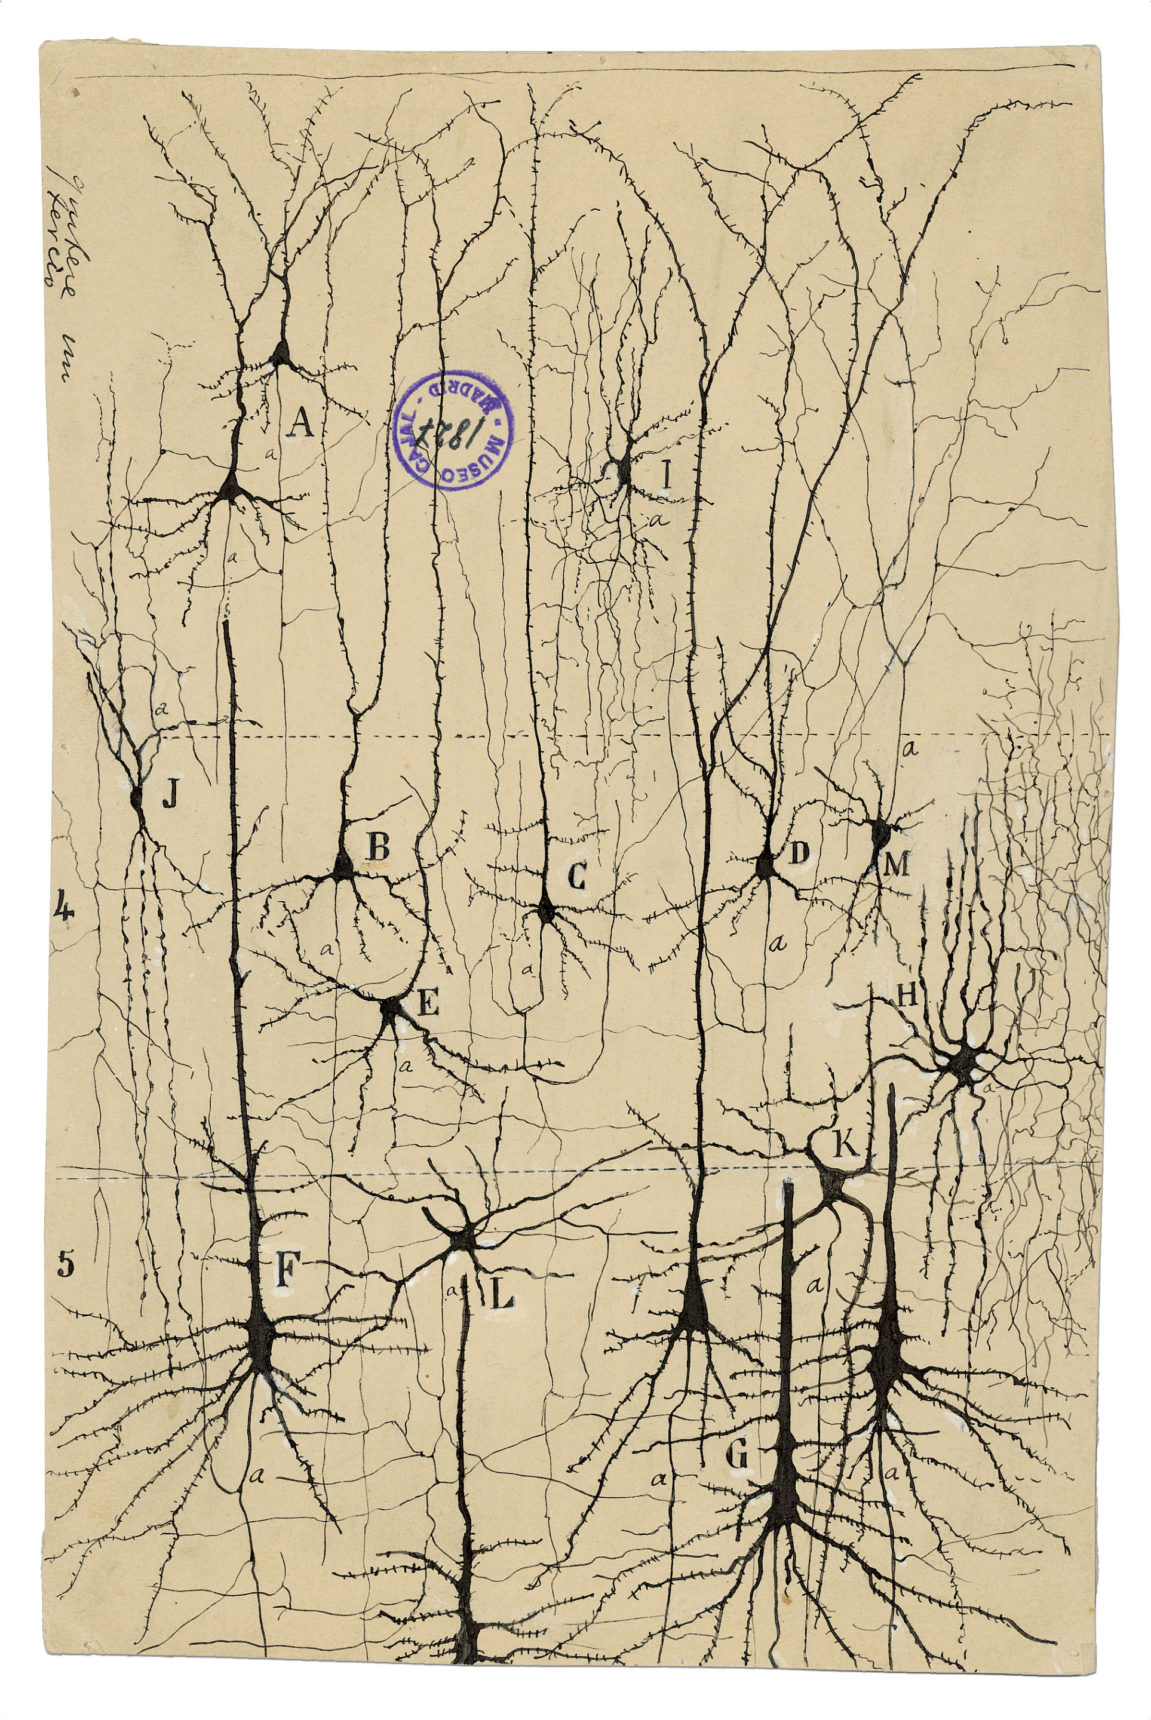
\includegraphics[width=3in]{figures/cajal_neuron.png}
    \caption{Drawing of neurons by Santiago Ram\'{o}n y Cajal in the late 19th century. Cajal was a pioneer of the field of neuroscience, and his insight that neurons are the discrete unit of computation and that communication between neurons happens through synapses became known as the neuron doctrine. In this drawing, note the dendrites (treelike structures toward the bottom), the cell body (the thick black part where the dendrites meet), and the axon (pointing up connecting to other neurons) of each neuron.}
    % https://www.quantamagazine.org/why-the-first-drawings-of-neurons-were-defaced-20170928/
    \label{fig:cajal_neuron}
\end{figure}

One important note is that an action potential is commonly referred to as ``all or nothing''. That is, the occurrence of a cell's spike is what is important, not the shape or duration of a spike. Moreover, after a spike is generated, the cell enters a short refractory period (on the order of milliseconds where it is biophysically impossible for the cell to fire another spike \citep{neuroscience_2nd_edition}. This absolute refractory period is followed by a relative refractory period where it is difficult, but not impossible, for the neuron to generate another spike. We will return to this later after discussing some of the ionic movements in neurons.

\subsection{Movement of Ions in the Neuron}
\label{sec:movement_of_ions}
The membrane potential in a neuron is a result of organic molecules in the brain such as sodium, potassium, calcium, and chloride (Na$^+$, K$^+$, Ca$^{2+}$, Cl$^-$). At rest, the inside of a neuron is more negatively charged than the substance outside, with the \textbf{resting potential} around -65 millivolts (mV) (though it is important to note that this number varies between different types/species of neuron). We will return to this value after mentioning how ions can travel in and out of the cell.

The impermeable lipid bilayer cell membrane in a neuron has proteins that allow ions to move in and out of the cell. These proteins are called \textbf{ion channels}. There are 2 types of channels, active channels and passive channels. The passive channels let the ions move freely into and out of the cell along the concentration gradient, while the active channels pump ions against the concentration gradient. One common type of active ion channels (and the one that is most pertinent to computational models of neuronal firing) is \textbf{voltage-gated ion channels}. These channels are closed when the cell is at resting potential and open in events where the membrane voltage changes.

Returning to the cell's resting potential, there are also special sodium-potassium pumps in the membrane that pump three Na$^+$ out of the cell while pumping two K$^+$ ions into the cell. This active process results in more positive charge outside of the cell, and thus maintaining a negative resting membrane potential to prevent the depolarization of the cell due to passive movement of ions along the concentration gradient. Thus, at resting potential, there is more Na$^+$ outside the cell, and more K$^+$ inside the cell. We will return to this fact later.

% https://courses.lumenlearning.com/boundless-biology/chapter/how-neurons-communicate/

\subsection{Neuronal Communication}
\label{sec:neuronal_communication}

% Cite https://www.ncbi.nlm.nih.gov/books/NBK11009/
As previously mentioned, when a presynaptic neuron's axon connects with a postsynaptic neuron's dendrite, a synapse is formed. The type of synapse relevant to our research (and the most common type of synapse in our brains) is a chemical synapse \citep{neuroscience_2nd_edition}. If two neurons are connected with a chemical synapse, the presynaptic neuron releases neurotransmitter molecules (stored in small sacs called vesicles) which flow across the synaptic cleft, the gap between the neurons. We will not focus on the various types of neurotransmitters, but commonly studied ones are acetylcholine and dopamine. The neurotransmitter molecules then bind to receptor molecules in the postsynaptic cell's membrane, opening voltage-gated ion channels and letting ions into the postsynaptic cell. Synapses can be excitatory or inhibitory. At \textbf{excitatory synapses}, positive ions enter the cell and result in \textbf{depolarization}, since the membrane potential difference is no longer large in magnitude. Incoming spikes at these synapses (excitatory postsynaptic potentials; EPSPs) increase the cell's membrane potential and makes it more likely to fire. At \textbf{inhibitory synapses}, the opposite is true. Inhibitory postsynaptic potentials (IPSPs) result in \textbf{hyperpolarization} (an increase in membrane potential; term comes from the fact that the membrane potential difference is growing large in magnitude) and make it less likely to fire. IPSPs and EPSPs can cancel each other out thus acting as a biological noise filter.
% http://techlab.bu.edu/resources/software_view/epsp_ipsp/index.html

If the postsynaptic neuron becomes sufficiently depolarized (this threshold is typically around -55 to -40 mV, though it varies), voltage-gated sodium channels in the cell membrane are opened, and by process of diffusion, an influx of positively charged sodium enter the neuron. (See above for more info on ion channels.) In Figure \ref{fig:membrane_v_during_spike} below, this corresponds to the steep increase in voltage \citep{neuroscience_2nd_edition}. The voltage peaks at around 40 mV, when the sodium channels close and the voltage-gated potassium channels open. Since potassium is highly concentrated inside the cell, potassium ions flow down the concentration gradient (i.e., out of the cell) which drops the cell's membrane potential. In Figure \ref{fig:membrane_v_during_spike} below, this corresponds to the steep drop in voltage. Potassium channels take longer to close than sodium channels, so K$^+$ ions continue to flow out of the neuron resulting in hyperpolarization (the slight dip below resting potential in Figure \ref{fig:membrane_v_during_spike}). The neuron is in a brief refractory period state where it cannot fire. The potassium channels then close and the previously-mentioned sodium-potassium pumps restore the resting potential. The Result of this process of depolarization (when sodium rushes in) and repolarization (when potassium rushes out) is propagated down the length of the axon and triggers the release of neurotransmitters into other synapses, which can thus cause the spiking of other neurons.

\begin{figure}[H]
    \centering
    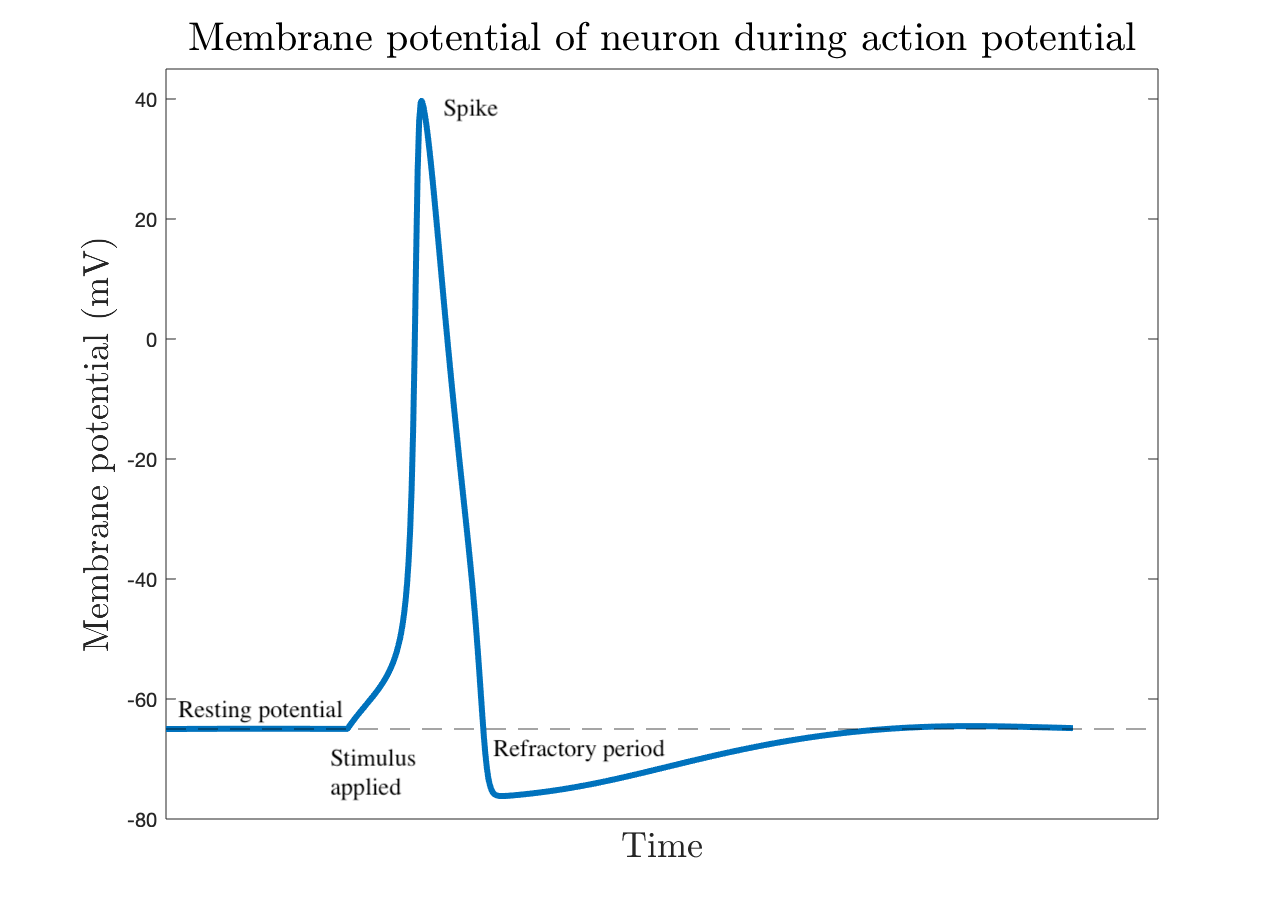
\includegraphics[width=5in]{figures/membrane_v_during_spike.png}
    \caption{Membrane potential during the firing of an action potential. Figure generated using Hodgkin-Huxley model (see section \ref{sec:hh_model}).}
    \label{fig:membrane_v_during_spike}
\end{figure}

It is also important to briefly mention the role of \textbf{synaptic plasticity}. This refers to the strengthening or weakening of synapses over time. A rough translation of Hebb's learning rule is ``neurons that fire together wire together'' referring to the fact synaptic strength changes in response to increases or decreases in activity \citep{synaptic-plasticity}. This forms the basis of learning and memory, which are core components of a nervous system. Much of the details of plasticity are not known, but the concept of plasticity is pivotal when developing computational models of networks of neurons.

% --------------------
\section{Computational Models of Neuronal Firing}
\label{sec:models}
% --------------------

As methods of collecting data of neuronal firing continue to improve, the field of computational neuroscience needs computational models to sort out and make sense of that data. Here we cover basic models used to model spiking neurons and discuss the uses and drawbacks of each model.

\subsection{Integrate and Fire Model}
\label{sec:integrate_and_fire}
Given all the information we have about neurons, it is essential that we are able to model said neurons to predict their behavior and uncover their secret ways of conducting actions and making decision with the chaos ensued by the firing of all neurons nearby. One of the earliest models of a neuron is the Integrate and Fire Model (IF model) which was first developed in 1907 by Louis Lapicque represented the neuron as a derivative of the law of capacitance \citep{lapicque}. This model relies on 3 key ideas to work. The first is that action potentials of a given neuron always have roughly the same form. Secondly, information was not transmitted through the different spike shapes, rather through the presence and absence of a spike. Finally, spikes can be reduced to 'events' that happen at a moment in time. Given those facts, the model consists of 3 main parts:

\begin{enumerate}[1)]
    \item A first-order linear differential equation to describe the evolution of the membrane potential with time,
    
    \begin{equation}
        \tau_m \frac{du}{dt} = - (u(t) - u_\text{rest}) + RI(t)
        \label{eq:integrate_and_fire}
    \end{equation}
    
    \item A threshold for spike firing,
    \item A voltage reset value for post-spike hyper-polarization.
\end{enumerate}

The differential equation represents the change in the membrane potential as a function of the input current and time. As the input current increases, the membrane potential increases up to a threshold. As the membrane potential crosses the threshold a spike is generated as a delta function (i.e., the voltage instantly spikes up). After the spike reaches its peak, the membrane potential is reset to a specific value below resting potential to simulate post-spike hyper-polarization.

While the model might appear to accurately predict the output of a neuron, it can only accurately predict the first spike, given that the input current is not a shunting current. The model regards action potentials as events in a time scale, and has no memory of previous spikes as we reset the membrane potential to a hard-coded value after every spike. The model also can't display adaptation for the same reason, unless we employ a filter. A filter used can be as simple as increasing the spiking threshold value for every spike generated. We can also add a ``leaking'' variable to resemble the membrane potential decay.

While the model lacks a lot in accurately modeling a neuron's biochemistry and biophysics, it does a great job in predicting spike firing times of a neuron if we employ all the aforementioned improvements. The integrate and fire model is great for constructing and simulating large populations of neurons as it is simple and doesn't cost much computationally to run these simulations.

All in all, the model with minor improvements for adaptation, memory and membrane potential decay is a great model to predict firing times, but alone without any improvements doesn't serve much use in our current time as we have much better models.

\subsection{Hodgkin-Huxley Model}
\label{sec:hh_model}
Another well-known model|perhaps the most well-known neuron model|is the Hodgkin-Huxley model (HH model). The model focuses on the relationship between the currents passing through the ion channels across the neuron membrane and the membrane potential \citep{hh}. The model was based on the giant squid axon, and then later expanded to model cortical cells in vertebrates and then in humans. It focused on the 3 types of ion channels, Na$^+$ channels that are responsible for the depolarization, K$^+$ channels that are responsible for the hyper-polarizing of the cell as well as a leak channel that represents the decay of the voltage, typically through the Cl$^-$ ion. The breakthrough of Hodgkin and Huxley was that they succeeded in measuring how the effective resistance of a channel changes as a function of voltage and time.

\begin{equation}
    C \frac{dV}{dt} = I(t) + \overline{g}_\text{K} n^4 (V - V_\text{K}) + \overline{g}_\text{Na} m^3h(V - V_\text{Na}) - \overline{g}_l(V - V_l)
    \label{eq:hodgkin_huxley}
\end{equation}

Variable definitions:
\begin{itemize}
    \item $C$: Capacitance of the membrane
    \item $V$: Current Membrane Potential
    \item $\frac{dV}{dt}$: Change in membrane potential
    \item $I(t)$: Time dependent input current
    \item $\overline{g}_\text{K}$, $\overline{g}_\text{Na}$, $\overline{g}_l$: conductances of the potassium, sodium, and leakage channels
    \item $V_\text{K}$, $V_\text{Na}$, $V_l$: Reversal potential of the potassium, sodium, and leakage channels
    \item $n$, $m$: Activation variables
    \item $h$: Inactivation variable
\end{itemize}

The leakage channel accounts for other channel types not explicitly defined. They modeled the flow of Na ions and K ions through the probability of the opening and closing of the channels, both passive and active, the conductance of the channels and their reversal potentials. For instance, the Na channel has activation and inactivation agents that are modelled by the variables $m$ and $h$. When the neuron is at the resting potential the value of \textit{m} is approximately 0. As the membrane potential increases above the resting potential, the gating variable $m$ increases. As $m$ increases, it activates the Na channel increasing the flow of the Na current. When the voltage returns to rest, $m$ decays back to 0 de-activating the channel. On the other hand, the variable $h$, has a large positive value at resting potential. As the membrane potential increase to a value above -40mV, $h$ approaches 0, therefore it inactivates the channel. If they voltage returns to 0, $h$ increases so that the channel undergoes de-inactivation. The model also accurately models the post-spike hyper-polarizing by the slow de-inactivation  of the Na channel caused by the $h$ variable. The conductance is measured through blocking said channel, and then injecting it with an input current and measuring its voltage. Upon dividing the input current with the voltage, we get the value for the conductance of the channel. The reversal potential is acquired through the use of the Nernst equation.

Unlike the Integrate-and-Fire Model, the Hodgkin-Huxley model excels when it comes to the accurately representing the biophysics and biochemistry of the neuron as we can easily account for additional ion channels simply by adding activation and inactivation channels for every ion type along with their reversal potential and channel conductance. If we know the dynamics of each channel type we can accurately model a neuron by knowing what channels it has by studying the composition of messenger RNA extracted from the neuron.

\subsection{Izhikevich Model}
\label{sec:izhikevich_model}

The model, published by Eugene M. Izhikevich reproduces spike outputs as accurate as the Hodgkin-Huxley model while sacrificing the biophysical plausibility \citep{izhikevich_model}. The model is based on on fitting the spike initiation dynamics of a cortical neurons such that the membrane potential is in mV and the time is in ms. Then upon reaching the apex of the spike, the membrane potential is reset to a hyper-polarizing reset value determined by prior spikes, followed by a recovery to the resting potential via the recoverability variable. Surprisingly, the model accurately reproduces the spiking behavior exhibited in real neurons, with accuracy approximate to that of the Hodgkin-Huxley model.

The model serves as a middle ground between the Integrate-and-Fire model (which is not complex enough to model many cortical spiking patterns as described in figure \ref{fig:izhikevich_spike_patterns}), and the Hodgkin-Huxley model, which is more complex and very biophysically accurate. While the Izhikevich model allows for easy analytical use, much like the integrate-and-fire model, the model is not biophysically accurate, and lacks in accurately simulating the neuron on a short time scale. The model is also difficult to tune to account for different types of neurons. It comes with 16 different presets of firing, but it's quite difficult to tune the model to represent a specific ``real'' neuron that is being worked on.

\begin{align}
    v' &= 0.04v^2 + 5v + 140 - u + I \label{eq:izhikevich_vprime} \\
    u' &= a(bv - u) \label{eq:izhikevich_uprime} \\
    % & \text{if } v \geq 30 \text{ mV},~ \text{then } \begin{pmatrix} v \\ u \end{pmatrix} = \begin{pmatrix} c \\ u+d \end{pmatrix} \label{eq:izhikevich_ifspike}
    & \text{if } v \geq 30 \text{ mV},~ \text{then } \begin{cases} v \leftarrow c \\ u \leftarrow u+d \end{cases} \label{eq:izhikevich_ifspike}
\end{align}

\begin{figure}[H]
    \centering
    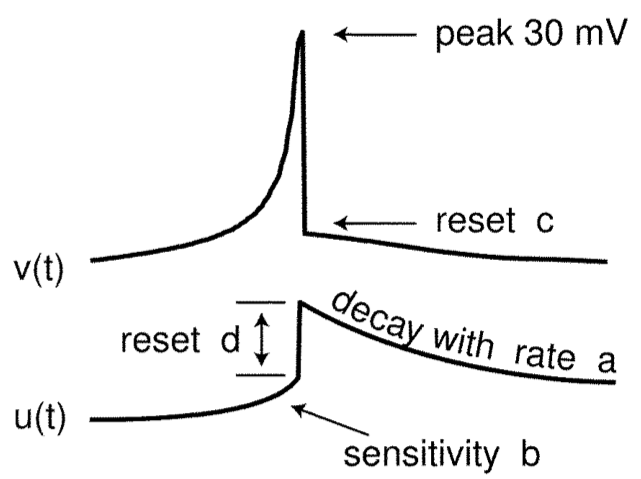
\includegraphics[width=3in]{figures/izhikevich_variable_descriptions.png}
    \caption{This figure shows the graph of $v(t)$, where it spikes, juxtaposed with the graph of $u(t)$. Notice the inverse relationship between $u$ and $v$ due to the variable $b$, because $u$ is being subtracted from the derivative of $v$. As $v$ increases up to the apex of the spike, $u$ increases slowly and at the firing time of the spike, $u$ is rest to the value $d$, and $v$ is reset to the value $c$. From there the recovery time from hyper-polarization of $v$ is dictated by the variable $a$. Figure from \cite{izhikevich_model}.}
    \label{fig:izhikevich_variable_descriptions}
\end{figure}

Variable Definitions:
\begin{itemize}
    \item $v'$: Change in membrane potential
    \item $u'$: Membrane potential recoverability (accounts for the activation of K+ ions and inactivation of Na+ ion)
    \item $a$: Time scale of the recovery variable 'u' (the larger the value, the faster the recovery) (insert something about proportionality)
    \item $b$: sensitivity of the recovery variable 'u' (larger values in low-threshold spiking dynamics and subthreshold oscillations)
    \item $c$: After spike rest value (Usually between -60 and -70 mv)
    \item $d$: After spike reset of the recovery variable (caused by Na and K conductances)
\end{itemize}

\begin{figure}[H]
    \centering
    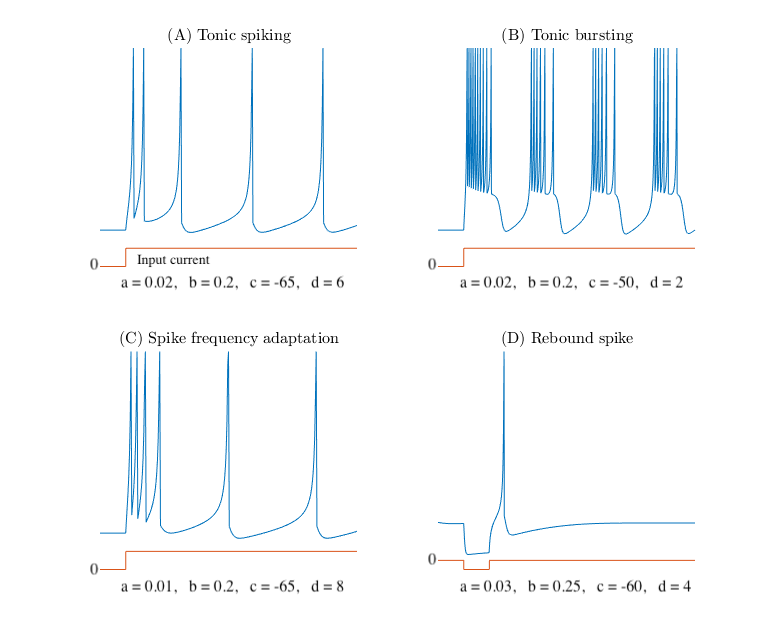
\includegraphics[width=6in]{figures/izhikevich_spike_patterns.png}
    \caption{Various patterns of spiking present in mammalian neocortex, modeled using the Izhikevich model. Membrane potential in blue and input current in orange underneath. Parameters for each model are listed below the plot. Note that these parameters have no direct biological counterpart as the parameters in the Hodgkin-Huxley model do. The Izhikevich parameters are simply tuned so the neuron exhibits biologically accurate patterns. Figure adapted from \cite{izhikevich_which_model}.}
    \label{fig:izhikevich_spike_patterns}
\end{figure}

\section{Methods}
\label{sec:methods}
We tested the following models: integrate-and-fire, Hodgkin-Huxley, Izhikevich (four models with patterns outlined in figure \ref{fig:izhikevich_spike_patterns}). Each model was fed a constant input current overlayed with white noise and 20 trials of spike trains were generated (where each spike train consisted of 50-100 spikes). We then computed the spike-triggered average (STA) and compared them across models. We also compared the voltage graphs for each of the models to see how spikes were visually different across the models. The timescale used is milliseconds.

% --------------------
\section{Results and Discussion}
\label{sec:results}
% --------------------
In this section we compare the inputs and outputs for the 3 models: the Integrate-and-Fire model, the Izhikevich model and the Hodgkin-Huxley model. The input current fed into the models is a series of white noise injected over a constant current value, measured in nA, while the voltage is what the models outputted as a result of the current, measured in mV. The timescale used is in ms.

\begin{figure}[H]
    \centering
    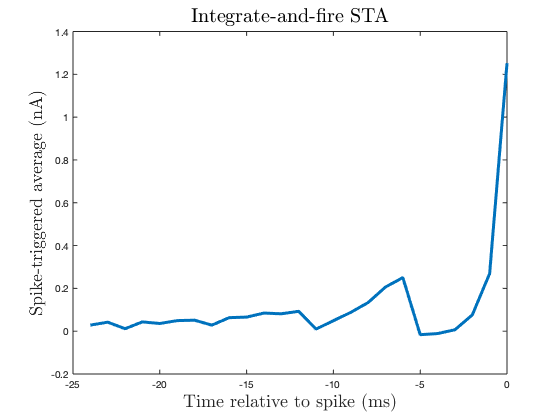
\includegraphics[width=5in]{figures/intfire_sta.png}
    \caption{Current STA for an integrate-and-fire model fed with white noise current.}
    \label{fig:intfire_sta}
\end{figure}

\begin{figure}[H]
    \centering
    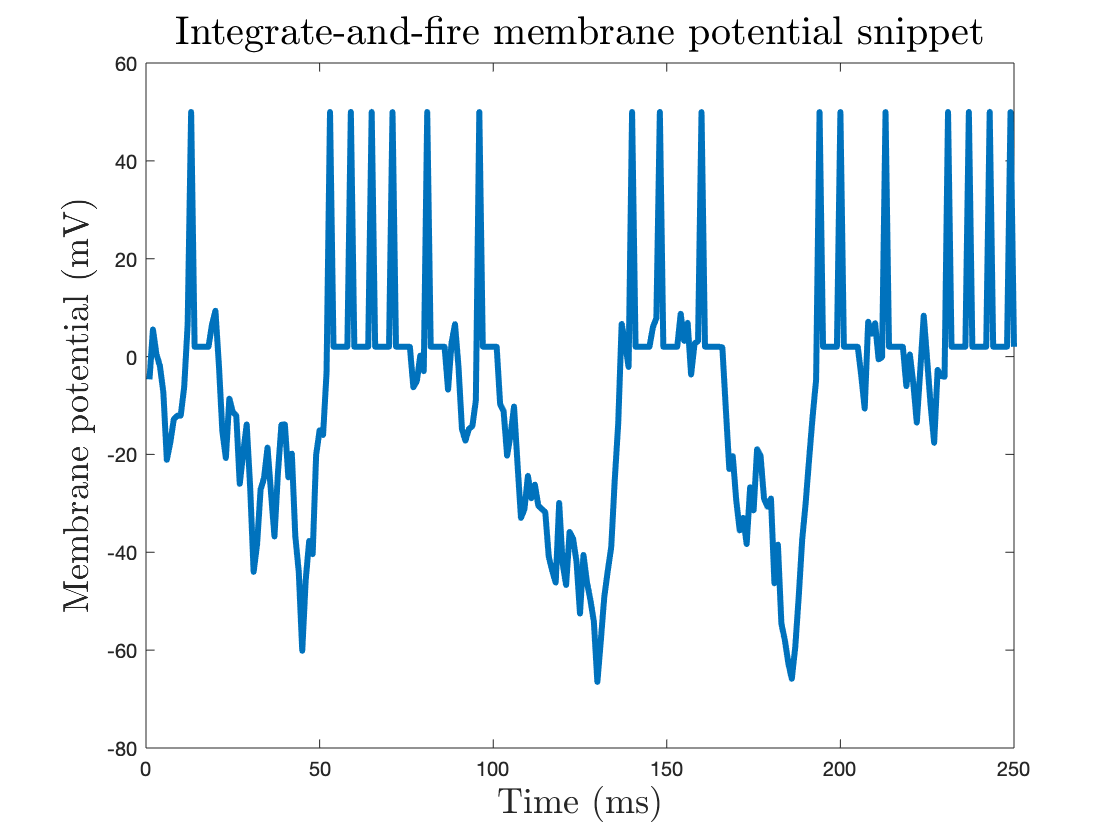
\includegraphics[width=5in]{figures/intfire_potential.png}
    \caption{Snippet from integrate-and-fire neuron model showing membrane potential over time when the model is fed with white-noise input.}
    \label{fig:intfire_potential}
\end{figure}

In figure \ref{fig:intfire_sta} we can see the spike-triggered average current for the Integrate-and-Fire model. This STA was generated by with in one trial. No further trials were needed as the Integrate-and-Fire model consistently generated spikes, and the model was very predictable even with the introduction of noise. We can see that a spike is being produced by the model at the exact moment where the input current increased, as the end of the STA doesn't decrease. This proves one of the flaws of the Integrate-and-Fire model; the biophysical implausibility. In real neurons, there is a time delay before the increase in current and production of spike, while this model doesn't display this property. 

\begin{figure}[H]
    \centering
    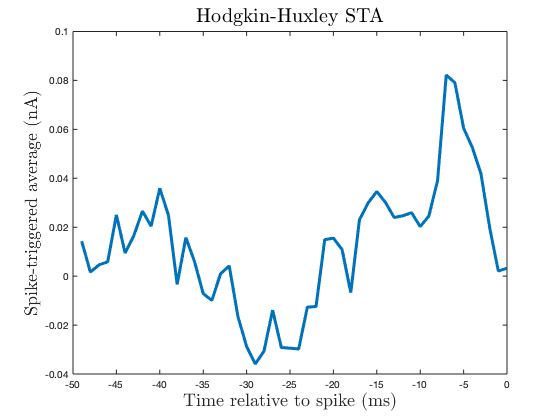
\includegraphics[width=4.5in]{figures/hh_sta_optimal.png}
    \caption{Current STA for an Hodgkin-Huxley model fed with white noise current.}
    \label{fig:hh_sta}
\end{figure}

In figure \ref{fig:hh_sta} we can see the spike-triggered average current for the Hodgkin-Huxley model. This STA was generated by computing 10 STAs of independent HH trials with different random white noise current, and averaging the 10 STAs together. On average, we can see that a spike produced by the model was preceded by a spike in current. Also note that there is a slight dip shortly before the spike, which looks visually similar to a differentiating linear kernel. This suggests that the neuronal model responds to sharp changes in current. The average STA shows the biophysical accuracy of the HH model. After the input reaches its peak value, there is a 10-15 ms time delay to fire a spike.

\begin{figure}[H]
    \centering
    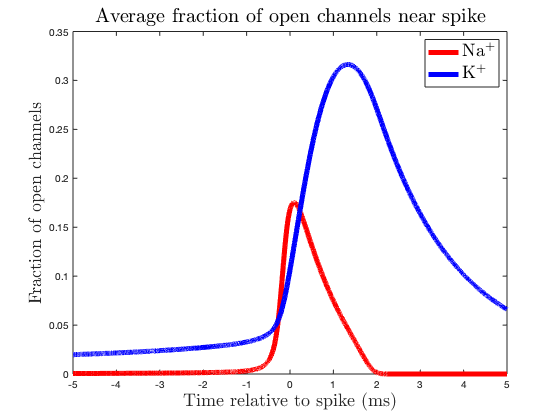
\includegraphics[width=4.5in]{figures/hh_fraction_channels_open.png}
    \caption{Fraction of open sodium and potassium channels in HH model. The K channels remain open for a longer period of time causing the post-spike hyper-polarization}
    \label{fig:hh_fraction_channels_open}
\end{figure}

\begin{figure}[H]
    \centering
    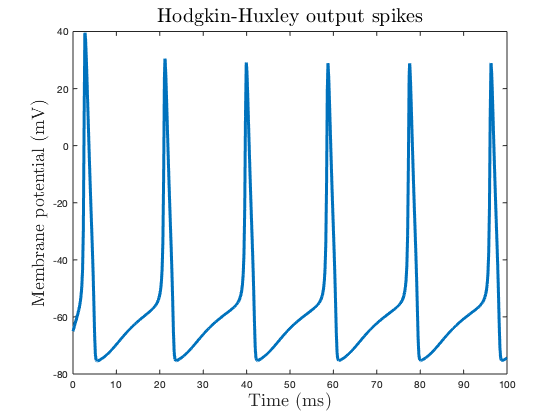
\includegraphics[width=4.5in]{figures/hh_spikes.png}
    \caption{Sample of the output spike train from HH model.}
    \label{fig:hh_spikes}
\end{figure}

In figure \ref{fig:hh_fraction_channels_open} we can see the biophysical accuracy of the Hodgkin-Huxley. As discussed in section \ref{sec:neuronal_communication}, the sodium channels open, resulting in a voltage spike, and then potassium channels open to re-polarize the membrane. The potassium channels stay open longer than the sodium channels, resulting in hyper-polarization and a short refractory period during which the neuron cannot spike.

\begin{figure}[H]
    \centering
    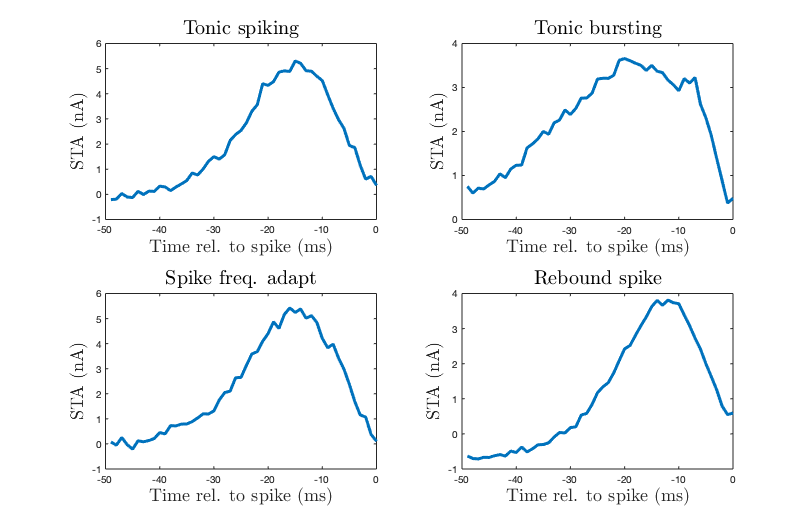
\includegraphics[width=6in]{figures/izhikevich_sta.png}
    \caption{Spike-triggered-average (STA) currents for various firing patterns on the Izhikevich model. See figure \ref{fig:izhikevich_spike_patterns} for spiking patterns. Interestingly the STAs for these various models are all fairly similar, with slightly varying widths. Further analysis methods beyond STA are likely needed to uncover more differences.}
    \label{fig:izhikevich_sta}
\end{figure}

In figure \ref{fig:izhikevich_sta} we can see how the Izhikevich serves as a middle ground between the integrate-and-fire model and the Hodgkin-Huxley model. All four STAs in figure \ref{fig:izhikevich_sta} have the same general shape, responding to a sharp increase in current. The STA looks like a combination of STAs from both models. Similar to the Hodgkin-Huxley model, we see a drop in current immediately prior to spiking, indicating that the neuron takes several milliseconds to fire once the membrane potential exceeds the threshold. However, unlike the Hodgkin-Huxley model, the STAs of all four Izhikevich models we investigated do not have a small drop prior to a spike characteristic of a edge detector or differentiating linear kernel.

% Include Adrienne's paper without actually citing it in-line
\nocite{computation-in-single-neuron-hh}

% --------------------
\section{Conclusion}
\label{sec:conclusion}
% --------------------
%https://www.izhikevich.org/publications/whichmod.pdf

As methods of of data collection improve and we are able to work with larger amounts of data, it is important that our models are efficient enough to process massive datasets with millisecond time accuracy. However, we must also maintain sufficient biological plausability, referring to how well our model matches the actual neurobiology of cells as discussed in section \ref{sec:background}. We refer to this as the biological plausibility and computational efficiency tradeoff. \footnote{Different machines with different compute capabilities will run models at different speeds, but a universal proxy for computational complexity is the number of floating point operations (FLOPS). A larger number of FLOPS means the model requires more computation at each iteration. The optimal model has a low number of FLOPS but is still biophysically accurate.}

Consider the Hodgkin-Huxley model as discussed in section \ref{sec:hh_model}. This model is incredibly biophysically accurate, with differential equations for ion channels and several degrees of freedom. However, this results in high computational complexity, making it hard to simulate large (thousands) quantities of neurons simultaneously. \footnote{Each step of a Hodgkin-Huxley model takes around 1200 FLOPS.} On the other end of the spectrum, we have the integrate-and-fire model as discussed in section \ref{sec:integrate_and_fire}. We have seen that although this model is not very biophysically accurate, it is very computationally efficient. \footnote{Each step of an integrate-and-fire model takes around 10 FLOPS.} Finally, we investigated the Izhikevich model, which can simulate spiking many spiking patterns of actual neurons found in cortex. While these spiking patterns can also be modeled with the HH model if the parameters are tuned properly, the Izhikevich is orders of magnitude faster and thus opens up the possibility to simulate thousands of spiking neurons with not a lot of computing power. \footnote{Each step of an Izhikevich model takes around 10-20 FLOPS} One tradeoff is the HH parameters are biophysically meaningful whereas the Izhikevich parameters are only proxies for firing dynamics.

Which model is best? In short, it depends on the problem. If the goal is to study how neuronal behavior varies when biophysical parameters (such as ion channel conductances and time constants), then the HH model will yield the most understandable results \citep{izhikevich_which_model}. However, if the goal is to efficiently model hundreds or even thousands of cortical neurons, then the integrate-and-fire or Izhikevich models will be better suited since we have seen these are more computationally efficient. The Izhikevich model, as we have also seen, accounts for more biophysical dynamics than the very simple integrate-and-fire model, and can generate spiking patterns akin to those that can be produced using the Hodgkin-Huxley model.

One possible future direction is to apply more complex analysis methods on top of the spike-triggered average. For example, we can compute the covariance matrices for stimuli around a spike and project spike-conditional stimuli along the leading two covariance modes, providing more information about what specific stimuli cause the neuronal models to spike. Another direction is to take advantage of simple models such as the Izhikevich model and use it to simulate a fully-connected network of hundreds of cortical spiking neurons. We could also fit a network of connected neurons to actual spike data and use it to perform more intricate analysis.

In conclusion, biologically plausible and computationally efficient models are highly relevant as methods of data collection improve, and we need to have at our disposal computational models that are able to efficiently model hundreds or even thousands of neurons.

\newpage
\section{Contributions}
\begin{itemize}
    \item Introduction (\ref{sec:intro}): Chase
    \item Background (\ref{sec:background}): Chase
    \item Movement of Ions (\ref{sec:movement_of_ions}): Chase and Ahmed
    \item Neuronal Communication (\ref{sec:neuronal_communication}): Chase
    \item Integrate-and-Fire Model (\ref{sec:integrate_and_fire}): Ahmed
    \item Hodgkin-Huxley Model (\ref{sec:hh_model}): Ahmed
    \item Izhikevich Model (\ref{sec:izhikevich_model}): Ahmed
    \item Methods (\ref{sec:methods}): Chase
    \item Results and Discussion (\ref{sec:results}): Chase and Ahmed
    \item Conclusion (\ref{sec:conclusion}): Chase
    \item \textsc{matlab} coding: Chase and Ahmed
\end{itemize}

% %%%%%%%%%%%%%%%%%%%%%%%%%%%%%%%%%%%%%%%%%%%%%%%%%%%%%%%%%%
% %%%%%%%%%%%%%%%%%%%%%%%%%%%%%%%%%%%%%%%%%%%%%%%%%%%%%%%%%%
% REFERENCES SECTION
% %%%%%%%%%%%%%%%%%%%%%%%%%%%%%%%%%%%%%%%%%%%%%%%%%%%%%%%%%%
% %%%%%%%%%%%%%%%%%%%%%%%%%%%%%%%%%%%%%%%%%%%%%%%%%%%%%%%%%%
\medskip

\bibliography{references}

\end{document}